\documentclass[a4paper]{article}
\usepackage[affil-it]{authblk}
\usepackage{amsthm,amsmath,amssymb}
\usepackage{geometry}
\usepackage{graphicx}
\usepackage{float}  
\usepackage{listings}  
\usepackage{xcolor}  
\geometry{margin=1.5cm, vmargin={0pt,1cm}}
\setlength{\topmargin}{-1cm}
\setlength{\paperheight}{29.7cm}
\setlength{\textheight}{25.3cm}
\newcommand{\QED}{\hfill\ensuremath{\square}}

\lstset{ 
    basicstyle=\ttfamily,
    keywordstyle=\color{blue},
    commentstyle=\color{gray},
    stringstyle=\color{red},
    numbers=left,
    numberstyle=\tiny\color{gray},
    stepnumber=1,
    numbersep=5pt,
    backgroundcolor=\color{white},
    showspaces=false,
    showstringspaces=false,
    showtabs=false,
    frame=single,
    tabsize=2,
    captionpos=b,
    breaklines=true,
    breakatwhitespace=false,
    escapeinside={\%*}{*)}
}

\begin{document}

% =================================================
\title{Numerical Analysis Project Report}

\author{Chen Wanqi 3220102895
  \thanks{Electronic address: \texttt{3220102895@zju.edu.cn}}}
\affil{Information and Computer Science 2201, Zhejiang University}

\date{\today}

\maketitle

\section{Implementing Linear Spline Functions \( S^0 \) in ppForm and BSpline Formats}

\subsection{Overview}
Taking PP-Form as an example, the following code is included in the spline constructor:
\begin{lstlisting}[language=C++]
if (spline_order == 1) {
        // Linear spline function S^0_1
        for(int j = 0; j < num_points - 1; ++j) {
            std::vector<double> x(2), y(2);
            x[0] = t[j]; x[1] = t[j + 1];
            y[0] = f[j]; y[1] = f[j + 1];
            polynomials[j] = Polynomial(x, y);
        }
        return PiecewisePolynomial(polynomials, t);
}
\end{lstlisting}
Simply set `spline\_order` to 1 to construct a linear spline.

\subsection{Test Results}
The test code is in `main.cpp`, as follows (some content is removed for brevity):
\begin{lstlisting}[language=C++]
double f1(double x) {
    return exp(x) - x * x + 1;
}

MathFunction f1_func(f1);
std::vector<MathFunction> f_v = {f1_func};

void check_P1() {
    
    PPSpline ppspline(1, 1, f_v, -1, 1, 40);
    BSpline bspline(1, 1, f_v, -1, 1, 40);
    ppspline.print();
    bspline.print();
    system("python3 plot.py output/check/P1_ppspline.txt");
    system("python3 plot.py output/check/P1_bspline.txt");
    stdout = original_stdout;
}
\end{lstlisting}
Running `main.cpp` will perform linear spline fitting on the target function \( f(x) = e^x - x^2 + 1 \) and output the results. The fitting results are plotted using a Python program, as shown below.
\begin{figure}[H]
    \centering
    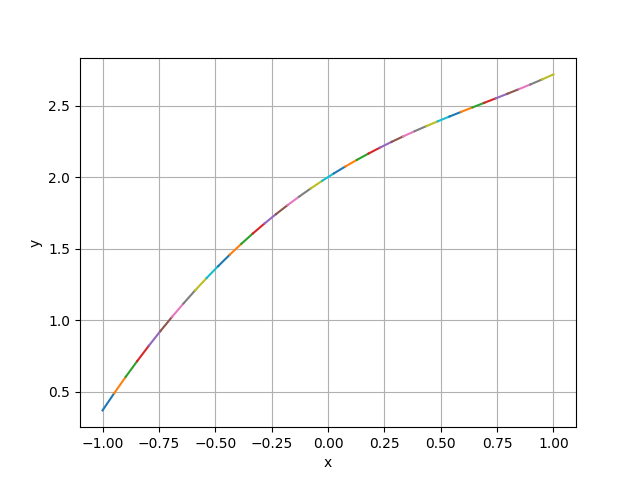
\includegraphics[width=0.45\textwidth]{./figure/check/P1_bspline.png}
    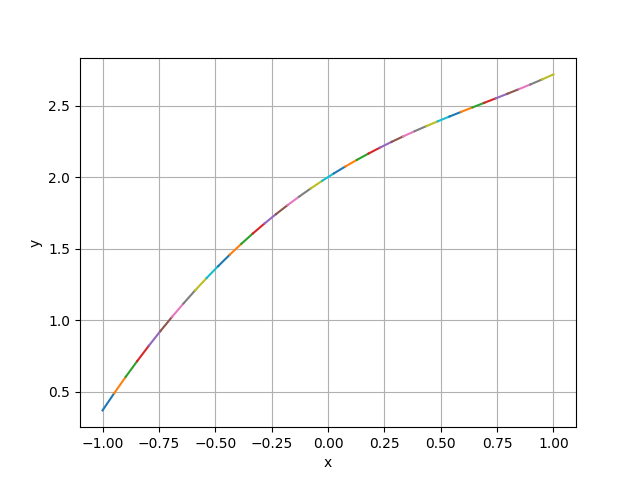
\includegraphics[width=0.45\textwidth]{./figure/check/P1_ppspline.png}
    \caption{Linear spline fitting results for BSpline and PPSpline}
\end{figure}

As can be seen, both spline fitting results are quite good. Thus, the first requirement is fulfilled!

\section{Deriving and Implementing Three Types of Cubic Splines in ppForm}

\subsection{Overview}

In the constructor of `PPSpline`, different treatments are applied for three types (actually five types) of boundary conditions.

\subsubsection{1. Complete Cubic Spline}
The boundary conditions are:
\[
s'(f; a) = f'(a), \quad s'(f; b) = f'(b)
\]
The system of equations is:
- The equations for internal nodes are consistent with the formula in the image:
  \[
  \lambda_{i-1} m_{i-1} + 2m_i + \mu_i m_{i+1} = 3[f[x_{i-1}, x_i] + f[x_i, x_{i+1}]]
  \]
  where \(i = 2, \dots, N-1\).
- Additional equations for boundary conditions:
  \[
  m_1 = f'(a), \quad m_N = f'(b)
  \]

\subsubsection{2. Cubic Spline with Specified Second Derivatives}
The boundary conditions are:
\[
s''(f; a) = f''(a), \quad s''(f; b) = f''(b)
\]
The system of equations is:
- The equations for internal nodes are consistent with the formula in the image:
  \[
  \lambda_{i-1} m_{i-1} + 2m_i + \mu_i m_{i+1} = 3[f[x_{i-1}, x_i] + f[x_i, x_{i+1}]]
  \]
  where \(i = 2, \dots, N-1\).
- Additional equations for boundary conditions (derived from the relationship between \(m\) and the second derivative):
  \[
  m_1 = \frac{6}{x_2 - x_1}(f[x_1, x_2] - f''(a)), \quad m_N = \frac{6}{x_N - x_{N-1}}(f[x_{N-1}, x_N] - f''(b))
  \]

\subsubsection{3. Natural Cubic Spline}
The boundary conditions are:
\[
s''(f; a) = 0, \quad s''(f; b) = 0
\]
The system of equations is:
- The equations for internal nodes are consistent with the formula in the image:
  \[
  \lambda_{i-1} m_{i-1} + 2m_i + \mu_i m_{i+1} = 3[f[x_{i-1}, x_i] + f[x_i, x_{i+1}]]
  \]
  where \(i = 2, \dots, N-1\).
- Additional equations for boundary conditions (since the second derivative is zero, indicating zero curvature):
  \[
  m_1 = 0, \quad m_N = 0
  \]

\subsubsection{4. Not-a-Knot Cubic Spline}
The boundary conditions are:
\[
s'''(f; x_2) \text{ is continuous}, \quad s'''(f; x_{N-1}) \text{ is continuous}
\]
The system of equations is:
- The equations for internal nodes are consistent with the formula in the image:
  \[
  \lambda_{i-1} m_{i-1} + 2m_i + \mu_i m_{i+1} = 3[f[x_{i-1}, x_i] + f[x_i, x_{i+1}]]
  \]
  where \(i = 2, \dots, N-1\).
- Additional equations for boundary conditions:
  - At \(x_2\):
    \[
    \frac{m_2 - m_1}{x_2 - x_1} = \frac{m_3 - m_2}{x_3 - x_2}
    \]
  - At \(x_{N-1}\):
    \[
    \frac{m_{N-1} - m_{N-2}}{x_{N-1} - x_{N-2}} = \frac{m_N - m_{N-1}}{x_N - x_{N-1}}
    \]

\subsubsection{5. Periodic Cubic Spline}
The boundary conditions are:
\[
s(f; b) = s(f; a), \quad s'(f; b) = s'(f; a), \quad s''(f; b) = s''(f; a)
\]
The system of equations is:
- The equations for internal nodes are consistent with the formula in the image:
  \[
  \lambda_{i-1} m_{i-1} + 2m_i + \mu_i m_{i+1} = 3[f[x_{i-1}, x_i] + f[x_i, x_{i+1}]]
  \]
  where \(i = 2, \dots, N-1\).
- Additional equations for boundary conditions:
  \[
  m_1 = m_N, \quad \frac{m_2 - m_1}{x_2 - x_1} = \frac{m_N - m_{N-1}}{x_N - x_{N-1}}
  \]

The specific code is too lengthy to display here.

\subsection{Test Results}
In `main.cpp`, three types of cubic splines are tested using the same function and randomly selected nodes as in the previous question:
\begin{lstlisting}[language=C++]
void check_P2() {

    // Randomly select 11 nodes in the interval [-1, 1]
    std::vector<double> t1;
    for (int i = 1; i <= 11; i++) {
        t1.push_back(-1 + 2.0 * rand() / RAND_MAX);
    }
    std::sort(t1.begin(), t1.end()); 
    
    FILE* original_stdout = stdout;
    PPSpline spline1(1, 3, f_v, t1, NATURAL_SPLINE);
    spline1.print();

    PPSpline spline2(1, 3, f_v, t1, CLAMPED);
    spline2.print();

    PPSpline spline3(1, 3, f_v, t1, PERIODIC_CONDITION);
    spline3.print();

}
\end{lstlisting}
After running, three cubic splines with different boundary conditions are generated, as shown below:
\begin{figure}[H]
    \centering
    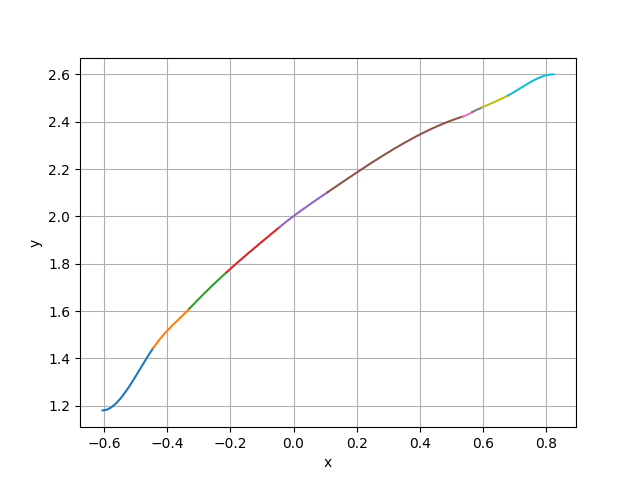
\includegraphics[width=0.45\textwidth]{./figure/check/P2_s23_clamped.png}
    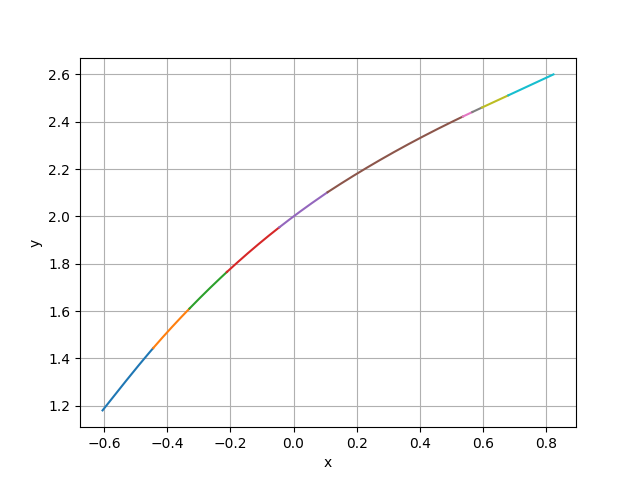
\includegraphics[width=0.45\textwidth]{./figure/check/P2_s23_natural.png}
    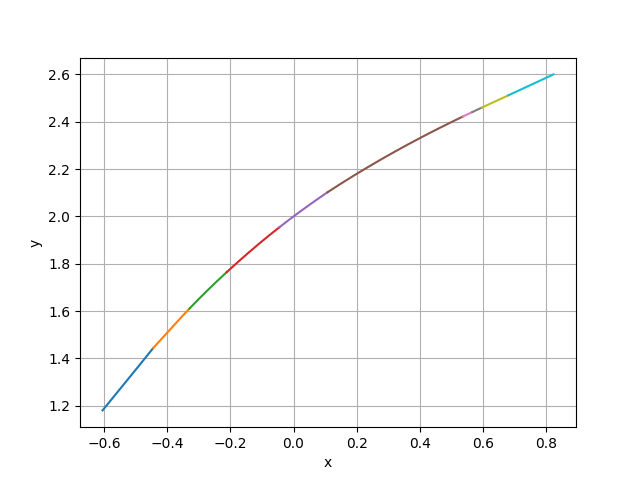
\includegraphics[width=0.45\textwidth]{./figure/check/P2_s23_periodic.png}
    \caption{Cubic spline fitting results for different boundary conditions}
\end{figure}

As can be seen, the cubic splines with different boundary conditions fit the target function well. Thus, the second requirement is fulfilled!

\section{Deriving and Implementing Three Types of Cubic Splines in BSpline Format}

\subsection{Overview \& Test Results}

Similar to `PPSpline`, the `BSpline` class also handles three types of boundary conditions differently. Here, we will not repeat the details, but only show the results.

\begin{figure}[H]
    \centering
    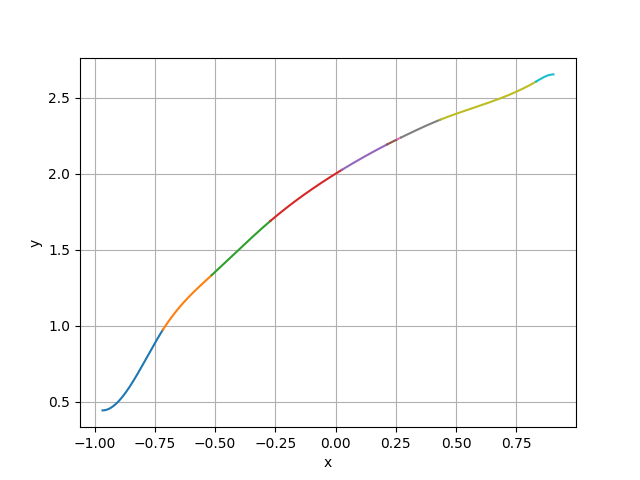
\includegraphics[width=0.45\textwidth]{./figure/check/P3_s23_clamped.png}
    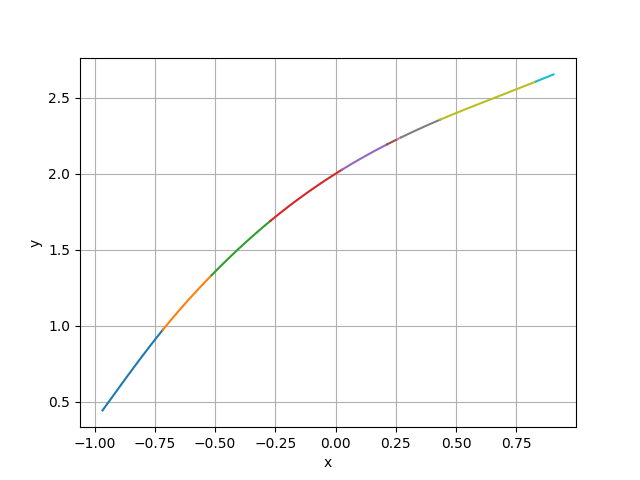
\includegraphics[width=0.45\textwidth]{./figure/check/P3_s23_natural.png}
    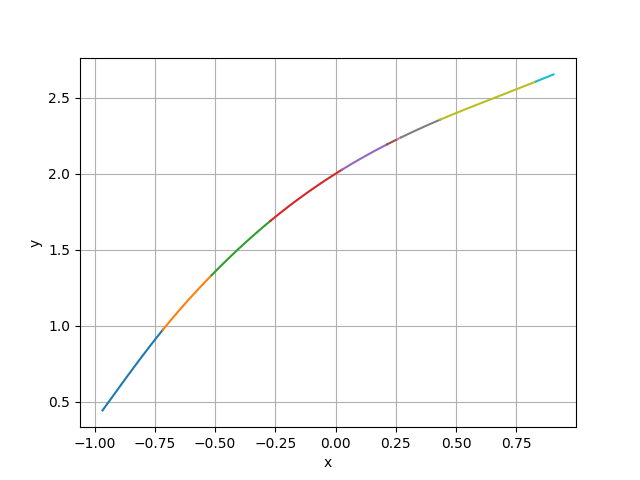
\includegraphics[width=0.45\textwidth]{./figure/check/P3_s23_periodic.png}
    \caption{Cubic spline fitting results for different boundary conditions in BSpline format}
\end{figure}

As can be seen, the cubic splines with different boundary conditions fit the target function well, and the results are within acceptable error margins compared to the PP splines. Thus, the third requirement is fulfilled!

\section{Verifying that Curves Obtained with the Same Interpolation Points and Boundary Conditions are Identical in ppForm and BSpline Formats}

\subsection{Overview \& Test Results}

In `main.cpp`, the results of Problem E are compared by plotting two results. For details, please refer to the report of Problem E. Here, we only show the results.

\begin{figure}[H]
    \centering
    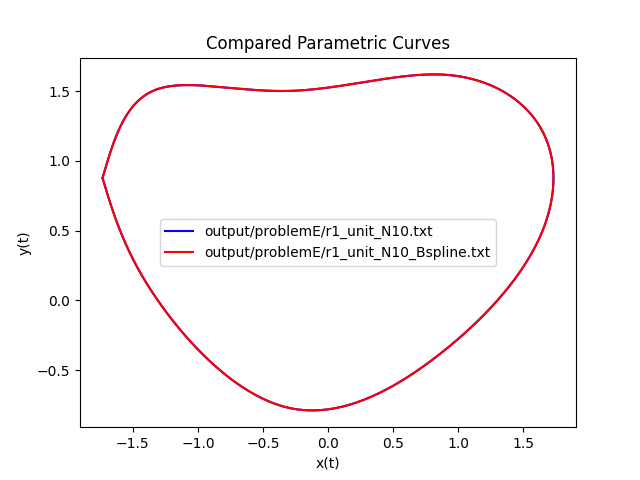
\includegraphics[width=0.45\textwidth]{./figure/check/P4_compare.png}
    \caption{Comparison of curves obtained in ppForm and BSpline formats}
\end{figure}

As can be seen, the two curves completely overlap. Therefore, it can be concluded that within acceptable error margins (often due to floating-point errors), the results obtained by both methods are consistent. This can also be seen from the previous question. Thus, the fourth requirement is fulfilled!

\section{BSpline Format Should Support Drawing Splines of Any Order and Any Nodes}

\subsection{Overview}

To achieve this functionality, a new constructor and a function to calculate the coefficients of basis functions of each order were added to the `BSpline` class, as follows:
\begin{lstlisting}[language=C++]
std::vector<std::vector<double>> evaluate_basis_coefficients(int i, int k) const;

BSpline(int dim, int order, const std::vector<double>& coefficients, 
        const std::vector<double>& time_points);
\end{lstlisting}
The former recursively calculates the coefficient arrays of basis functions in each segment interval, sorted from high to low, by inputting \(i\) and \(n\).

The latter constructs a `BSpline` object using the coefficient arrays calculated by the former, as well as the given coefficient weights and nodes.

\subsection{Test Results}

In `main.cpp`, the `BSpline` class was tested as follows:
\begin{lstlisting}[language=C++]
void check_P5() {
    // Randomly generate a sequence of nodes N=11
    std::vector<double> t1;
    for (int i = 1; i <= 11; i++) {
        t1.push_back(-0.5 + 2.0 * rand() / RAND_MAX);
    }
    std::sort(t1.begin(), t1.end()); 

    std::vector<double> coefficients;
    for (int i = 1; i <= 14; i++) {
        coefficients.push_back(-1.0 + 2.0 * rand() / RAND_MAX);
    }
    BSpline spline1(1, 4, coefficients, t1);
    spline1.print();
}
\end{lstlisting}
Randomly generate coefficients and nodes to construct a `BSpline` object, as shown below:

\begin{figure}[H]
    \centering
    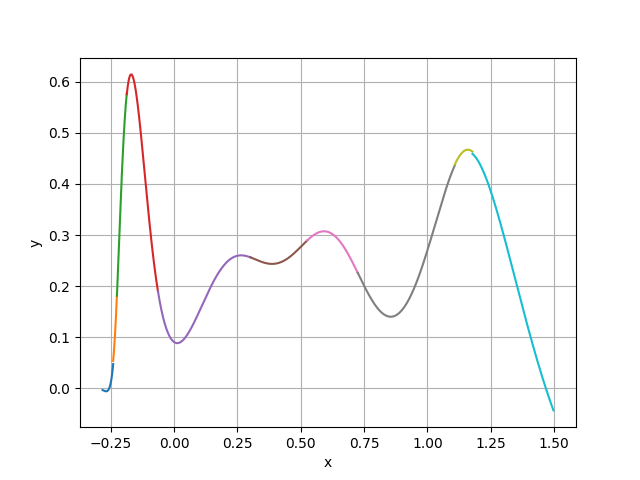
\includegraphics[width=0.45\textwidth]{./figure/check/P5_bspline.png}
    \caption{BSpline fitting results with random coefficients and nodes}
\end{figure}

As can be seen, the fitting is not very good...

\section{Implementing Spline Curve Fitting on a Plane}

\subsection{Overview}

Select several points from a given curve and use the previously implemented spline fitting methods for fitting.

The following tasks are all about curve fitting, so no additional tests are performed.

\section{Implementing Spline Curve Fitting on a Sphere}

\subsection{Overview}

First, create a sphere with center (0,0,1) and radius 1 in space. Connect the North Pole (0,0,2) with a point on the sphere, and there will be an intersection with the xOy plane, thus achieving a mapping from the sphere to the plane. For several points on the sphere, we first map them to the plane, then use the previously implemented spline fitting methods for fitting, and finally map the fitting results back to the sphere.

\subsection{Test Results}

Randomly selected several points on the sphere and performed fitting, as shown below:
\begin{figure}[H]
    \centering
    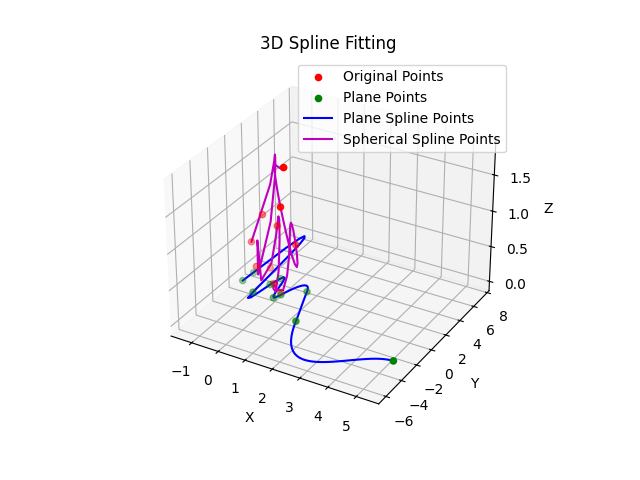
\includegraphics[width=0.45\textwidth]{./figure/Sphere/spline_fitting_all.png}
    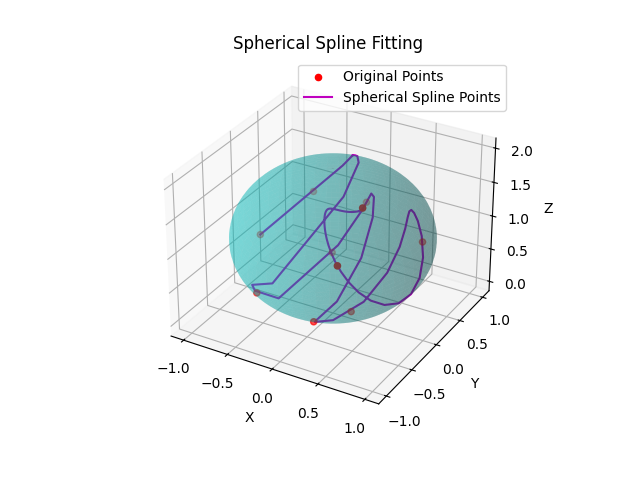
\includegraphics[width=0.45\textwidth]{./figure/Sphere/spline_fitting_spherical.png}
    \caption{Spline fitting results on the sphere}
\end{figure}

As can be seen, the fitting effect is quite good. Thus, the seventh requirement is fulfilled!

\section{Problem A}

\subsection{Test Code}

\begin{lstlisting}[language=C++]
// Define MathFunction f(x) = 1/(1 + 25 * x^2)
double f(double x) {
    return 1.0 / (1 + 25 * x * x);
}

MathFunction f_func(f);

std::vector<int> Ns = {6, 11, 21, 41, 81};

int main () {
    for (int i = 0; i < Ns.size (); ++ i) {
        freopen (("output/problemA/N_" + std :: to_string (Ns [i]) + ".txt").c_str (), "w", stdout);
        std::vector<MathFunction> f_v = {f_func};
        PPSpline spline (1, 3, f_v, -1.0, 1.0, Ns [i], CLAMPED); 
        spline.print ();
        double maxError = 0.0;
        for (int j = 0; j < Ns [i] - 1; ++ j) {
            
            double x = -1.0 + j * 2.0 / (Ns [i] - 1) + 1.0 / (Ns [i] - 1);
            double error = fabs (spline (x)[0] - f (x));
            if (error > maxError)
                maxError = error;
        }
        std :: cerr << "Error (N = " << Ns [i] << "): " << maxError << std :: endl;
        fclose (stdout);
    }
    return 0;
}
\end{lstlisting}

\subsection{Test Results}

\begin{verbatim}
Error (N = 6): 0.422378
Error (N = 11): 0.02052
Error (N = 21): 0.00316891
Error (N = 41): 0.000586206
Error (N = 81): 0.000293076
\end{verbatim}

\begin{figure}[H]
    \centering
    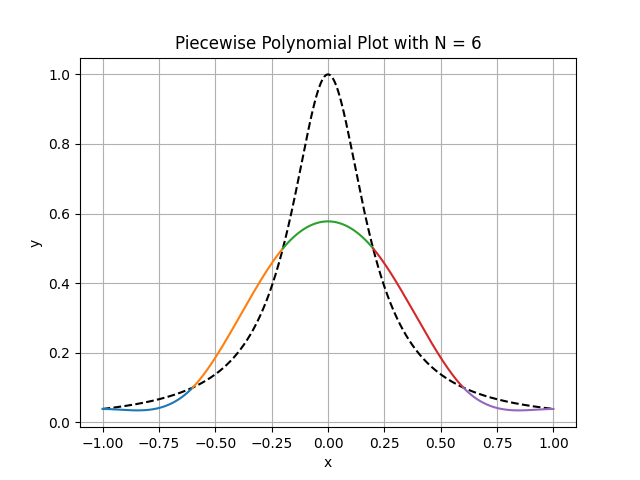
\includegraphics[width=0.45\textwidth]{./figure/problemA/N_6.png}
    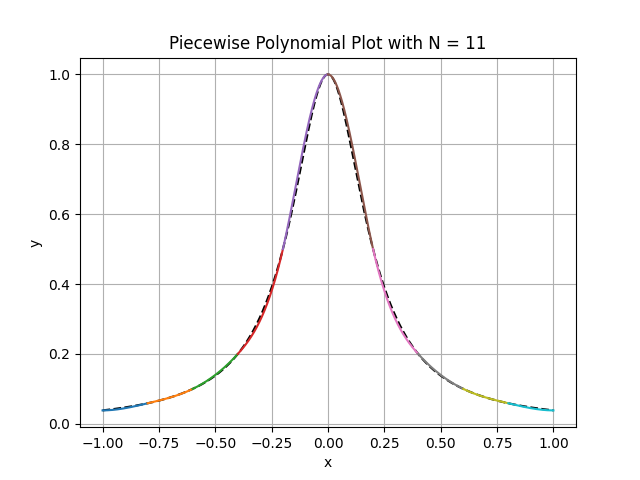
\includegraphics[width=0.45\textwidth]{./figure/problemA/N_11.png}
    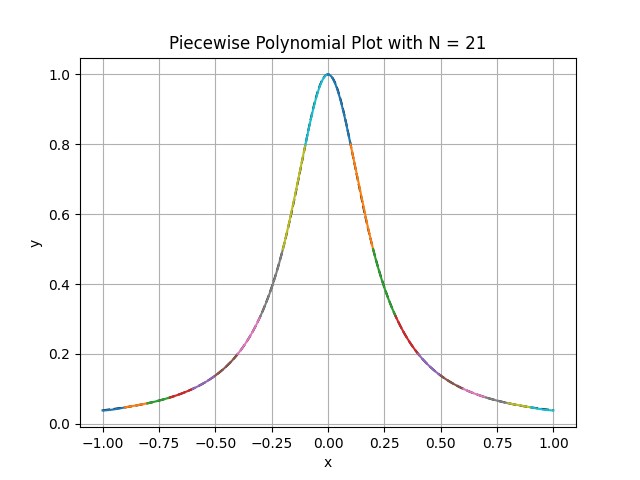
\includegraphics[width=0.45\textwidth]{./figure/problemA/N_21.png}
    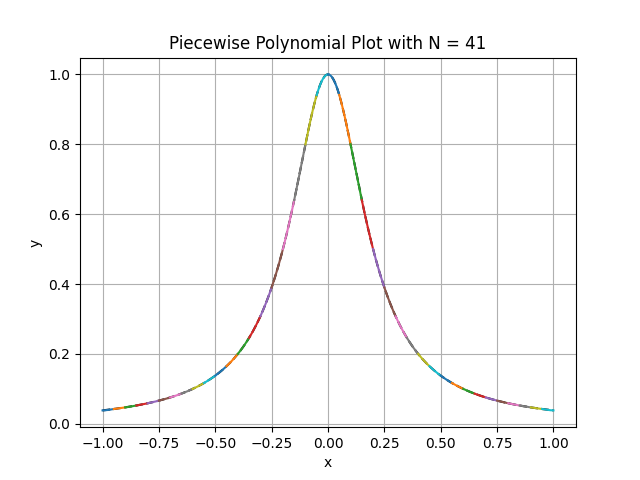
\includegraphics[width=0.45\textwidth]{./figure/problemA/N_41.png}
    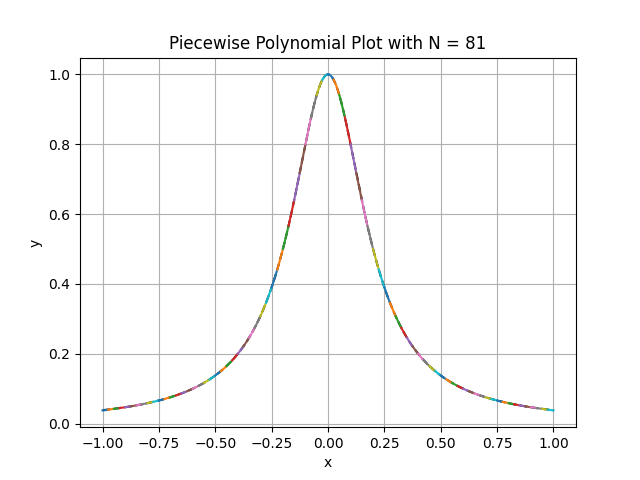
\includegraphics[width=0.45\textwidth]{./figure/problemA/N_81.png}
    \caption{Spline fitting results for different N values in Problem A}
\end{figure}

The fitting effect of the curve is quite good.

\section{Problem C}

\subsection{Test Code}

\begin{lstlisting}[language=C++]
double f(double x) {
    return 1 / (1 + x * x);
}

MathFunction f_func(f);

int main() {
    std::vector<MathFunction> f_v = {f_func};
    std::vector<double> t1;
    for (int i = 1; i <= 11; i++) {
        t1.push_back(i - 6);
    }
    freopen("output/problemC/s23.txt", "w", stdout);
    BSpline spline1(1, 3, f_v, t1, NATURAL_SPLINE);
    spline1.print();
    fclose(stdout);

    std::vector<double> t2;
    for (int i = 1; i <= 10; i++) {
        t2.push_back(i - 5.5);
    }
    freopen("output/problemC/s12.txt", "w", stdout);
    BSpline spline2(1, 2, f_v, t2);
    spline2.print();
    fclose(stdout);

    return 0;
}
\end{lstlisting}

\subsection{Test Results}
\begin{figure}[H]
    \centering
    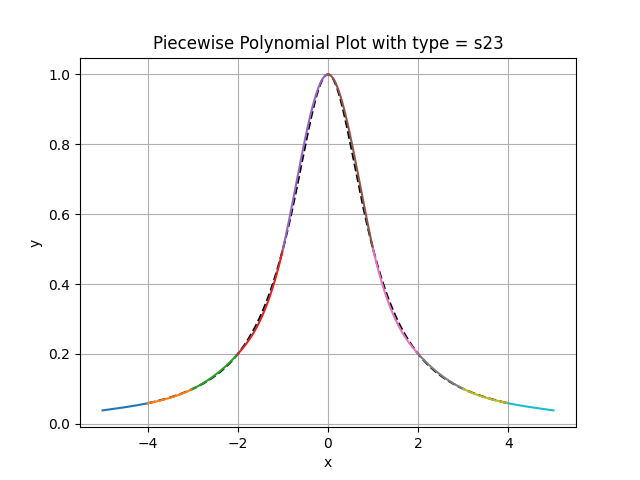
\includegraphics[width=0.45\textwidth]{./figure/problemC/s23.png}
    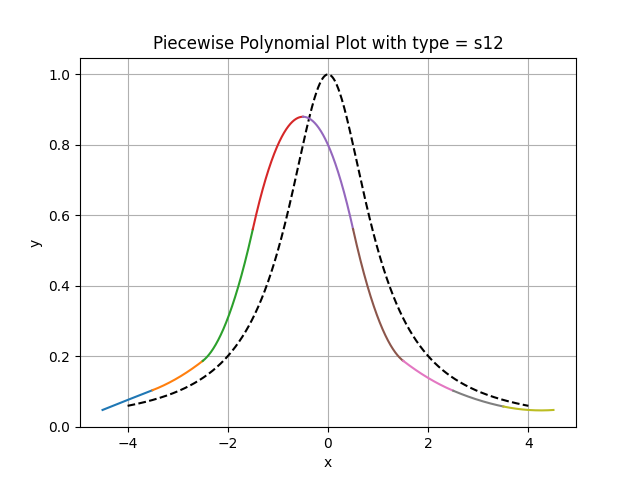
\includegraphics[width=0.45\textwidth]{./figure/problemC/s12.png}
    \caption{Spline fitting results for Problem C}
\end{figure}

\section{Problem D}

\subsection{Test Code}

\begin{lstlisting}[language=C++]
double f(double x) {
    return 1 / (1 + x * x);
}

MathFunction f_func(f);

int main() {
    std::vector<MathFunction> f_v = {f_func};
    std::vector<double> t1;
    for (int i = 1; i <= 11; i++) {
        t1.push_back(i - 6);
    }
    freopen("output/problemD/s23.txt", "w", stdout);
    BSpline spline1(1, 3, f_v, t1, NATURAL_SPLINE);
    spline1.print();
    fclose(stdout);

    std::vector<double> t2;
    for (int i = 1; i <= 10; i++) {
        t2.push_back(i - 5.5);
    }
    freopen("output/problemD/s12.txt", "w", stdout);
    BSpline spline2(1, 2, f_v, t2);
    spline2.print();
    fclose(stdout);

    std::vector<double> CPS = {-3.5, -3, -0.5, 0, 0.5, 3, 3.5};
    for (int i = 0; i < CPS.size(); ++i) {
        double err1 = fabs(spline1(CPS[i])[0] - f(CPS[i]));
        double err2 = fabs(spline2(CPS[i])[0] - f(CPS[i]));
        std::cerr << "Error at " << CPS[i] << ":\n";
        std::cerr << "Cubic spline: " << err1 << "\n";
        std::cerr << "Quadratic spline: " << err2 << "\n";
    }

    return 0;
}
\end{lstlisting}

\subsection{Test Results}

\begin{verbatim}
Error at -3.5:
Cubic spline: 0.000789971
Quadratic spline: 0.027888
Error at -3:
Cubic spline: 8.32667e-17
Quadratic spline: 0.037931
Error at -0.5:
Cubic spline: 0.0205306
Quadratic spline: 0.0797511
Error at 0:
Cubic spline: 1.11022e-16
Quadratic spline: 0.2
Error at 0.5:
Cubic spline: 0.0205306
Quadratic spline: 0.239278
Error at 3:
Cubic spline: 1.94289e-16
Quadratic spline: 0.0245283
Error at 3.5:
Cubic spline: 0.000789971
Quadratic spline: 0.0185731
\end{verbatim}

\section{Problem E}

Implement the heart-shaped curve required by the problem \[ r_2(t) = (x(t), y(t)) = (\sin t + t \cos t, \cos t - t \sin t), t \in [0, 6\pi] \] and \[ r_3(t) = (x(t), y(t), z(t)) = (\sin(u(t)) \cos(v(t)), \sin u(t) \sin v(t), \cos u(t)), t \in [0, 2\pi] \] three curves, where the third curve \( u(t) = \cos t \), \( v(t) = \sin t \). The three curves should be fitted using cumulative chordal length and equidistant nodes, and the fitting effects of these two nodes should be compared.

\subsection{Test Results}
Due to space limitations, only the fitting results for \( n = 40 \) are shown. For other results, please check the `figure/problemE` folder.
\begin{figure}[H]
    \centering
    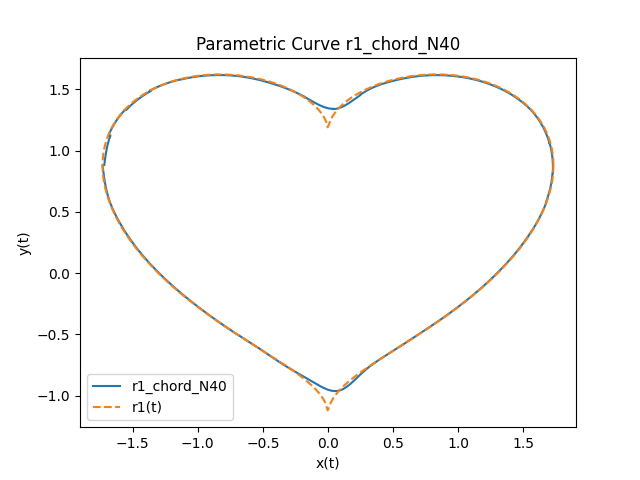
\includegraphics[width=0.45\textwidth]{./figure/problemE/r1_chord_N40.png}
    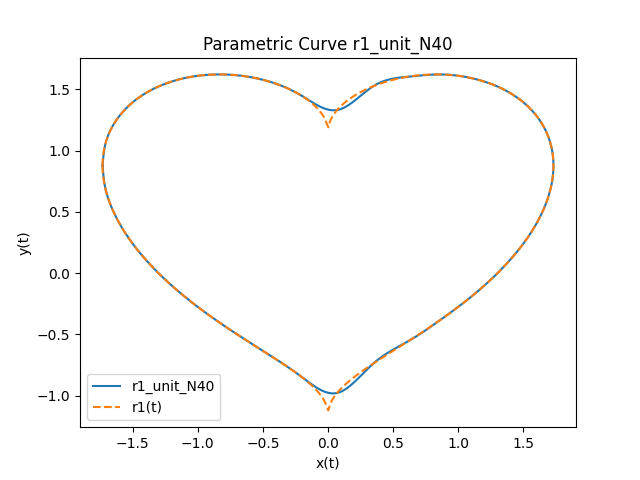
\includegraphics[width=0.45\textwidth]{./figure/problemE/r1_unit_N40.png}
    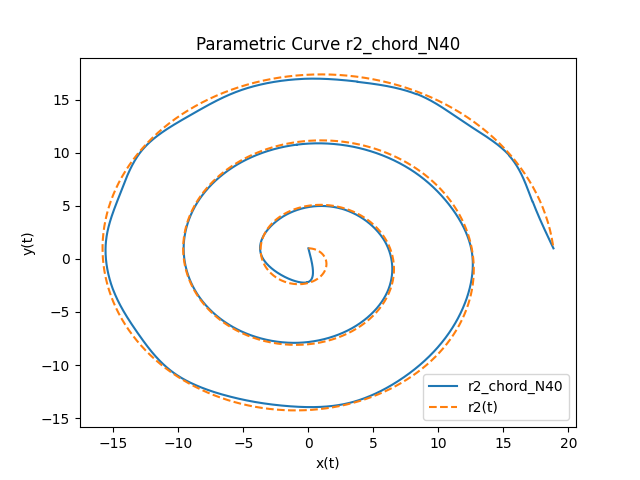
\includegraphics[width=0.45\textwidth]{./figure/problemE/r2_chord_N40.png}
    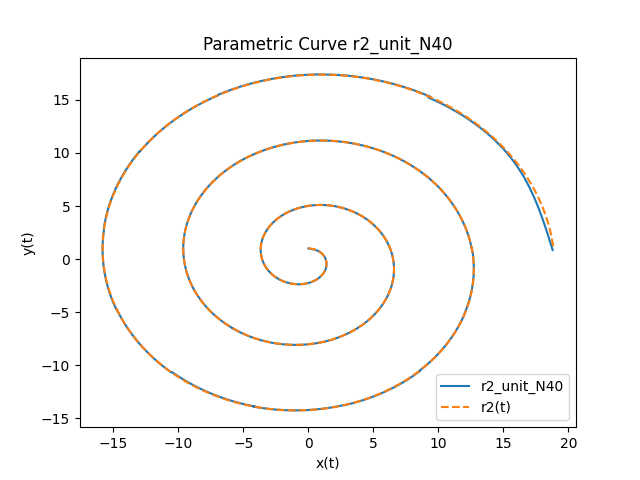
\includegraphics[width=0.45\textwidth]{./figure/problemE/r2_unit_N40.png}
    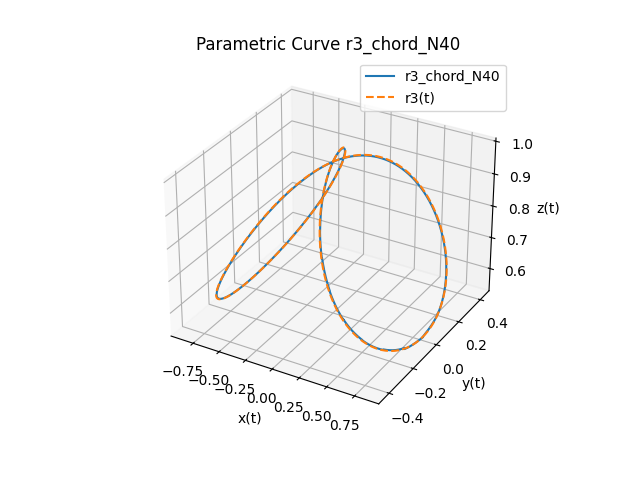
\includegraphics[width=0.45\textwidth]{./figure/problemE/r3_chord_N40.png}
    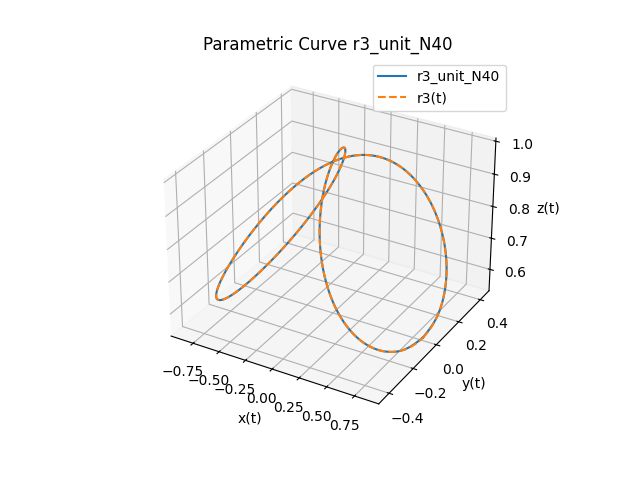
\includegraphics[width=0.45\textwidth]{./figure/problemE/r3_unit_N40.png}
    \caption{Fitting results for Problem E with \( n = 40 \)}
\end{figure}

\section{Bonus}

\subsection{Implementation of jsoncpp}

Implemented spline fitting controlled by a JSON file to avoid repeated compilation.

The JSON file is written according to the following rules:
\begin{lstlisting}[]
{
    "spline_type": "BSpline",                       // Spline type, can be "BSpline" or "PPSpline"
    "dimension": 2,                                 // Spatial dimension, number of variables to be fitted, 1 can represent y=f(x), 2 can represent x=x(t), y=y(t), and so on
    "order": 3,                                     // Order k
    "method": "uniform",                            // Point selection method, including uniform, chordal, custom, special
    "interval": [-1, 1],                            // Fill in when the point selection method is "uniform" or "chordal"
    "num_interval": 10,                             // Fill in when the point selection method is "uniform" or "chordal"
    "time_points": [0, 1, 2, 3, 4],                 // Node sequence (fill in when the point selection method is "custom" or "special")
    "coefficients": [1, 2, 3, 4, 5, 6, 7, 8],       // Coefficient vector (fill in when the point selection method is "special")
    "boundary_condition": "NATURAL_SPLINE",         // Boundary condition, can be "NATURAL_SPLINE", "CLAMPED", "PERIODIC_CONDITION"
    "da": 0.0,                                      // Derivative value of the boundary condition
    "db": 0.0                                       // Derivative value of the boundary condition
}
\end{lstlisting}
Run `src/Json/test.cpp` to control spline fitting through the JSON file.

\subsection{More Function Examples for Testing}

\subsubsection{Selected Five Functions}

Linear function, quadratic function, higher-order function, exponential function, and logarithmic function, trigonometric function.

The plots are as follows:
\begin{figure}[H]
    \centering
    \includegraphics[width=0.45\textwidth]{./figure/test/func_plot.png}
    \caption{Fitting results for various functions}
\end{figure}

It can be seen that the fitting results are very good.

\subsection{Convergence Order Analysis}

\subsubsection{Third-Order B-Spline (Natural Boundary Condition)}

Under the natural boundary condition, the second derivative of the approximating function is set to zero at both endpoints, i.e., \(N''(a) = 0\), \(N''(b) = 0\), to ensure the smoothness of the interpolation.

Consider the target function \(f(x)\) as a continuously differentiable function of the fourth order, i.e., \(f \in C^4\), and use a third-order B-spline for interpolation or approximation. When the nodes are uniformly distributed and the node spacing is \(h\), the approximation error can be expressed as:

\[
\| f(x) - S(x) \|_\infty = C \cdot h^4 \cdot \max_{x \in [a, b]} |f^{(4)}(x)| + \mathcal{O}(h^5)
\]

where \(\| \cdot \|_\infty\) denotes the maximum norm, \(C\) is a constant related to the spline basis function, and \(h\) is the node spacing. This result indicates that the global error convergence rate of the third-order B-spline is of the fourth order.

The error \(f(x) - S(x)\) can be decomposed into two parts: the error between the target function and the interpolation function \(f(x) - I[f](x)\), and the error between the interpolation function and the B-spline function \(I[f](x) - S(x)\). The first part of the error comes from the construction of the interpolation polynomial, with a convergence order of four; the second part is due to the smoothness of the B-spline basis function and the reasonable distribution of nodes, and its order effect can be ignored. Therefore, the overall error convergence order is still dominated by the first part, remaining at four.

\subsubsection{Third-Order PP-Spline (Natural Boundary Condition)}

In each subinterval \([x_i, x_{i+1}]\), the third-order PP-spline \(S(x)\) is a cubic polynomial. Let \(x \in [x_i, x_{i+1}]\), the spline is expressed as:
\[
S(x) = a_i + b_i(x-x_i) + c_i(x-x_i)^2 + d_i(x-x_i)^3,
\]
where \(a_i, b_i, c_i, d_i\) are coefficients uniquely determined in each interval by the spline interpolation conditions and natural boundary conditions. Since \(S(x)\) satisfies piecewise \(C^2\) continuity over all intervals, its first derivative \(S'(x)\) and second derivative \(S''(x)\) are continuous at the nodes, and the natural boundary conditions \(S''(a) = 0\) and \(S''(b) = 0\) provide additional constraints.

Consider the function \(f(x)\) within the interval \([x_i, x_{i+1}]\):
\[
f(x) = f(x_i) + f'(x_i)(x-x_i) + \frac{f''(x_i)}{2}(x-x_i)^2 + \frac{f^{(3)}(x_i)}{6}(x-x_i)^3 + R_4(x),
\]
where \(R_4(x)\) is the higher-order remainder term of the Taylor expansion, given by:
\[
R_4(x) = \frac{f^{(4)}(\xi)}{24}(x-x_i)^4, \quad \xi \in [x_i, x_{i+1}].
\]

The interpolation construction of the third-order spline \(S(x)\) ensures that \(S(x_i) = f(x_i)\), and the first and second derivatives at the nodes approximate the corresponding values of the function \(f(x)\). The dominant term of the error \(E(x) = f(x) - S(x)\) comes from the mismatch of the third derivatives of \(f(x)\) and \(S(x)\). Through higher-order analysis, the error estimate within each subinterval is:
\[
E(x) = \frac{f^{(4)}(\xi)}{384}h^4 + O(h^5), \quad \xi \in [x_i, x_{i+1}].
\]

Here, the main term of the error is proportional to the fourth derivative of the function \(f^{(4)}(\xi)\) and the fourth power of the node spacing \(h\).

To calculate the global error over the entire interval, consider the maximum value of \(E(x)\) over the interval. Since the nodes are uniformly distributed, the integral error can be approximated by the sum of the segment errors, and the overall error is:
\[
\|E(x)\|_\infty = \max_{x \in [a, b]} |E(x)| \leq C \cdot h^4 \cdot \|f^{(4)}(x)\|_\infty,
\]
where \(C\) is a constant related to the spline construction, and \(\|f^{(4)}(x)\|_\infty = \max_{x \in [a, b]} |f^{(4)}(x)|\). Therefore, the convergence order of the third-order PP-spline under natural boundary conditions is \(O(h^4)\).

\end{document}